\documentclass[simplex.tex]{subfiles}
% NO NEED TO INPUT PREAMBLES HERE
% packages are inherited; you can compile this on its own
\begin{document}
\subsection{Network Dependence Test via Diffusion Maps and MGC} 
%Deciphering the association between network structures and corresponding nodal attributes of interest is a core problem in network science. We propose a new nonparametric procedure for testing dependence between network topology and nodal attributes, via diffusion maps and \texttt{MGC}. Specifically, under an exchangeable graph, we verify that the diffusion maps provide a set of conditionally independent multivariate coordinates for the nodes, which can be combined with \texttt{MGC} (or in general, any distance-based correlation measures) to yield consistent statistic for network dependence testing. In simulation, the new approach achieves superior testing performance under a variety of common network models than existing benchmarks. The diffusion maps provides a robust metric compared to adjacency matrix or geodesic distance, while \texttt{MGC} can better capture nonlinear dependencies, with their combined advantages shown in Figure~\ref{fig:threeSBM}.  
%
%\begin{figure}[h!]
%\begin{cframed}
%		\centering
%		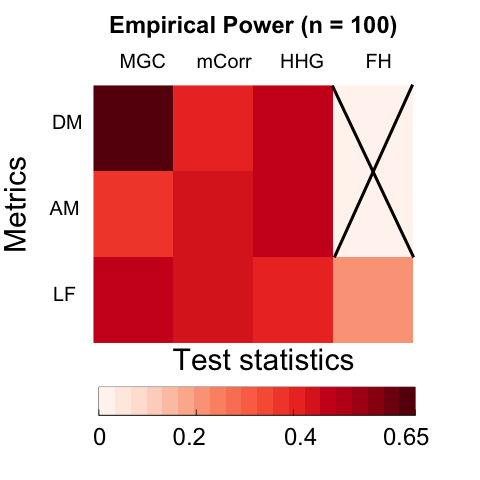
\includegraphics[width=0.6\textwidth]{../../figs/ThreeSBM.png}
%		\caption{Power comparison for all possible combinations of metrics and correlation measure, under the stochastic block model with three blocks. \texttt{MGC} with the diffusion maps (DM) yields the best power, comparing to using other metrics like adjacency matrix (AM), latent factors (LF), and other test statistics like distance correlation (mcorr), Heller-Heller-Gorfine (HHG) test, or Fosdick and Hoff (FH) method.}
%		\label{fig:threeSBM}
%		\end{cframed}
%\end{figure}
%
%%In order to show that \texttt{MGC} combined with diffusion maps as a network metrics perform better even in the case arbitrary noisy is added to edges or the attributes in real data, we are doing an experiment on brain network with physical locations as nodal attributes. Our proposed method not only detects the dependence between network topology and nodal attributes but also helps us to reveal possibly diverse dependence patterns through multiscale correlation maps or multiscale statistics as a function of diffusion time.
%
%This month we made significant progress in writing the manuscript and improving the exposition. The current draft was submitted to ASA Nonparametric Statistics Section Student Paper Awards, and we are notified as finalists for awards and special presentation section in the Joint Statistical Meeting this year. 
%
\end{document}
